\PassOptionsToPackage{table}{xcolor}
\documentclass[12pt,aspectratio=169]{beamer}

\usetheme{Warsaw}
\useoutertheme[subsection=false]{smoothbars}

\usepackage{graphicx}
\usepackage{booktabs}
\usepackage{tabularx}
\usepackage{amsmath}
\usepackage{xcolor}
\usepackage{array}
\usepackage{ragged2e}
\usepackage{natbib}

\newcolumntype{L}[1]{>{\RaggedRight\arraybackslash}p{#1}}
\newcolumntype{Y}{>{\RaggedRight\arraybackslash}X}

% Colors
\definecolor{UMGreenDark}{RGB}{122,153,112}
\definecolor{UMGreenLight}{RGB}{232,235,199}
\definecolor{UMOrangeDark}{RGB}{214,112,38}

\setbeamercolor*{palette secondary}{fg=black,bg=UMGreenLight}
\setbeamercolor*{palette tertiary}{fg=UMGreenLight,bg=UMOrangeDark}
\setbeamercolor*{palette quaternary}{fg=black,bg=UMGreenDark}
\setbeamercolor*{item projected}{bg=UMOrangeDark,fg=white}

\setbeamercolor{titlelike}{bg=UMOrangeDark}
\setbeamercolor{block title}{bg=UMGreenDark}
\setbeamercolor{block body}{bg=UMGreenLight}
\setbeamercolor{structure}{fg=black}

\setbeamertemplate{footline}[frame number]

% Title info
\title{Toward Vision-Guided Pick-and-Place for Tabletop Humanoid Manipulation}
\author{Dewan Tauhid Rahman}
\institute{Department of Computer Science \\ University of Miami}
\date{\today}

\begin{document}

\begin{frame}
  \titlepage
\end{frame}

\begin{frame}{Outline}
  \tableofcontents
\end{frame}

% ------------------------------------------------
\section{Introduction}

\begin{frame}{Motivation}
\begin{itemize}
    \item Many robotic systems work well only in structured settings with predefined objects and tasks, rather than in open-ended human environments \cite{Kober2013RLRobotics,Kasaei2021LifelongServiceRobots}.
    \item Real-world environments are less stable: layouts change, new objects appear, and uncertainty affects both perception and control \cite{Kasaei2021LifelongServiceRobots,Zheng2025EmbodiedManipSurvey}.
    \item For humanoid robots, a key capability is \textbf{perception-to-manipulation}: detecting an object, estimating how to grasp it, and executing manipulation reliably \cite{Zheng2025EmbodiedManipSurvey}.
    \item This project studies that capability in a controlled tabletop setting using the Fourier GR-1 humanoid as a first step toward more adaptive embodied behavior.
\end{itemize}
\end{frame}

\begin{frame}{Problem Setting}
\begin{block}{Long-term vision}
Build an integrated visuomotor system in which the robot:
\begin{enumerate}
    \item observes a scene,
    \item identifies a target object,
    \item estimates the object information needed for grasping,
    \item executes grasp-and-place behavior robustly.
\end{enumerate}
\end{block}

\vspace{0.35cm}
\begin{itemize}
    \item Current focus: controlled tabletop pick-and-place.
    \item Immediate goal: establish reliable manipulation on hardware.
    \item Longer-term goal: integrate this manipulation stack with a perception module that can adapt to new objects over time \cite{Kasaei2021LifelongServiceRobots,Zhou2024CILSurvey}.
\end{itemize}
\end{frame}

\begin{frame}{Why It Is Challenging}
\begin{itemize}
    \item \textbf{Sim-to-real gap:} policies trained in simulation often degrade on physical hardware \cite{Tobin2017DomainRandomization}.
    \item \textbf{Manipulation sensitivity:} contact-rich behaviors are highly affected by geometry, friction, and alignment error \cite{Tobin2017DomainRandomization,Zheng2025EmbodiedManipSurvey}.
    \item \textbf{Pipeline fragility:} if perception shifts or object pose changes, downstream manipulation can fail \cite{Kasaei2021LifelongServiceRobots,Zheng2025EmbodiedManipSurvey}.
    \item \textbf{Over-engineering risk:} scripted systems often depend on heuristic waypoints, thresholds, and fixed assumptions.
\end{itemize}
\end{frame}

% ------------------------------------------------
\section{Background}

\begin{frame}{Visuomotor Manipulation}
\footnotesize
\centering
\renewcommand{\arraystretch}{1.08}
\setlength{\tabcolsep}{4pt}

\begin{table}[h]
\centering
\begin{tabularx}{0.96\textwidth}{L{3.0cm} L{3.8cm} Y}
\toprule
\multicolumn{1}{c}{\textbf{Theme}} &
\multicolumn{1}{c}{\textbf{What Prior Work Shows}} &
\multicolumn{1}{c}{\textbf{Limitation}} \\
\midrule

CLIPort~\cite{Shridhar2022CLIPort}
& Semantic grounding with spatial manipulation
& Still assumes fixed perception during task execution \\[0.28em]

PerAct~\cite{Shridhar2023PerAct}
& Structured 3D action representations for multi-task manipulation
& Mostly evaluated under fixed object categories and benchmark settings \\[0.28em]

RT-1 / Octo / Diffusion Policy~\cite{Brohan2022RT1,Ghosh2024Octo,Chi2023DiffusionPolicy}
& Large-scale policy learning improves robustness and generalization
& Continual adaptation after deployment is not central \\
\bottomrule
\end{tabularx}
\end{table}

\vspace{-0.1cm}
\textbf{Takeaway:} Visuomotor manipulation is strong, but it still largely relies on fixed perception and fixed deployment distributions.
\end{frame}

\begin{frame}{Continual Perception and Adaptation}
\footnotesize
\centering
\renewcommand{\arraystretch}{1.08}
\setlength{\tabcolsep}{4pt}

\begin{table}[h]
\centering
\begin{tabularx}{0.96\textwidth}{L{3.0cm} L{3.8cm} Y}
\toprule
\multicolumn{1}{c}{\textbf{Area}} &
\multicolumn{1}{c}{\textbf{What Exists}} &
\multicolumn{1}{c}{\textbf{What Is Missing}} \\
\midrule

LwF / iCaRL~\cite{LiHoiem2016LwF,Rebuffi2017iCaRL}
& Mitigate forgetting during incremental learning
& Mostly validated on vision benchmarks, not robot behavior \\[0.28em]

LoRA~\cite{Hu2021LoRA}
& Efficient adaptation through lightweight modules
& Efficient updating does not guarantee stable manipulation \\[0.28em]

Lifelong robotics~\cite{Kasaei2021LifelongServiceRobots,Meng2025RoboticLifelongRL}
& Continuous learning is required for long-term autonomy
& Coupling adaptive perception and action remains limited \\
\bottomrule
\end{tabularx}
\end{table}

\vspace{-0.1cm}
\textbf{Takeaway:} Continual learning supports perception, but embodied deployment remains much less developed.
\end{frame}

\begin{frame}{Research Gap}
\footnotesize
\centering
\renewcommand{\arraystretch}{1.08}
\setlength{\tabcolsep}{4pt}

\begin{table}[h]
\centering
\begin{tabularx}{0.96\textwidth}{L{3.0cm} L{3.8cm} Y}
\toprule
\multicolumn{1}{c}{\textbf{Theme}} &
\multicolumn{1}{c}{\textbf{What Prior Work Shows}} &
\multicolumn{1}{c}{\textbf{Limitation}} \\
\midrule
Manipulation systems~\cite{Shridhar2023PerAct,Brohan2022RT1,Ghosh2024Octo}
& Strong task execution and policy learning
& Usually assumes fixed perception and stable object knowledge \\[0.28em]

Continual perception~\cite{Hu2021LoRA,Rebuffi2017iCaRL,Zhou2024CILSurvey}
& Incremental knowledge update with reduced forgetting
& Rarely evaluated through downstream grasping or placement \\[0.28em]

Embodied adaptation~\cite{Kasaei2021LifelongServiceRobots,Meng2025RoboticLifelongRL}
& Calls for perception and action to evolve together
& A stable perception-to-action interface is still missing \\
\bottomrule
\end{tabularx}
\end{table}

\vspace{-0.1cm}
\textbf{Takeaway:} The key gap is stable coordination between evolving perception and downstream action.
\end{frame}

% ------------------------------------------------
\section{Methodology}

\begin{frame}{End-to-End System Diagram}
    \begin{figure}
        \centering
        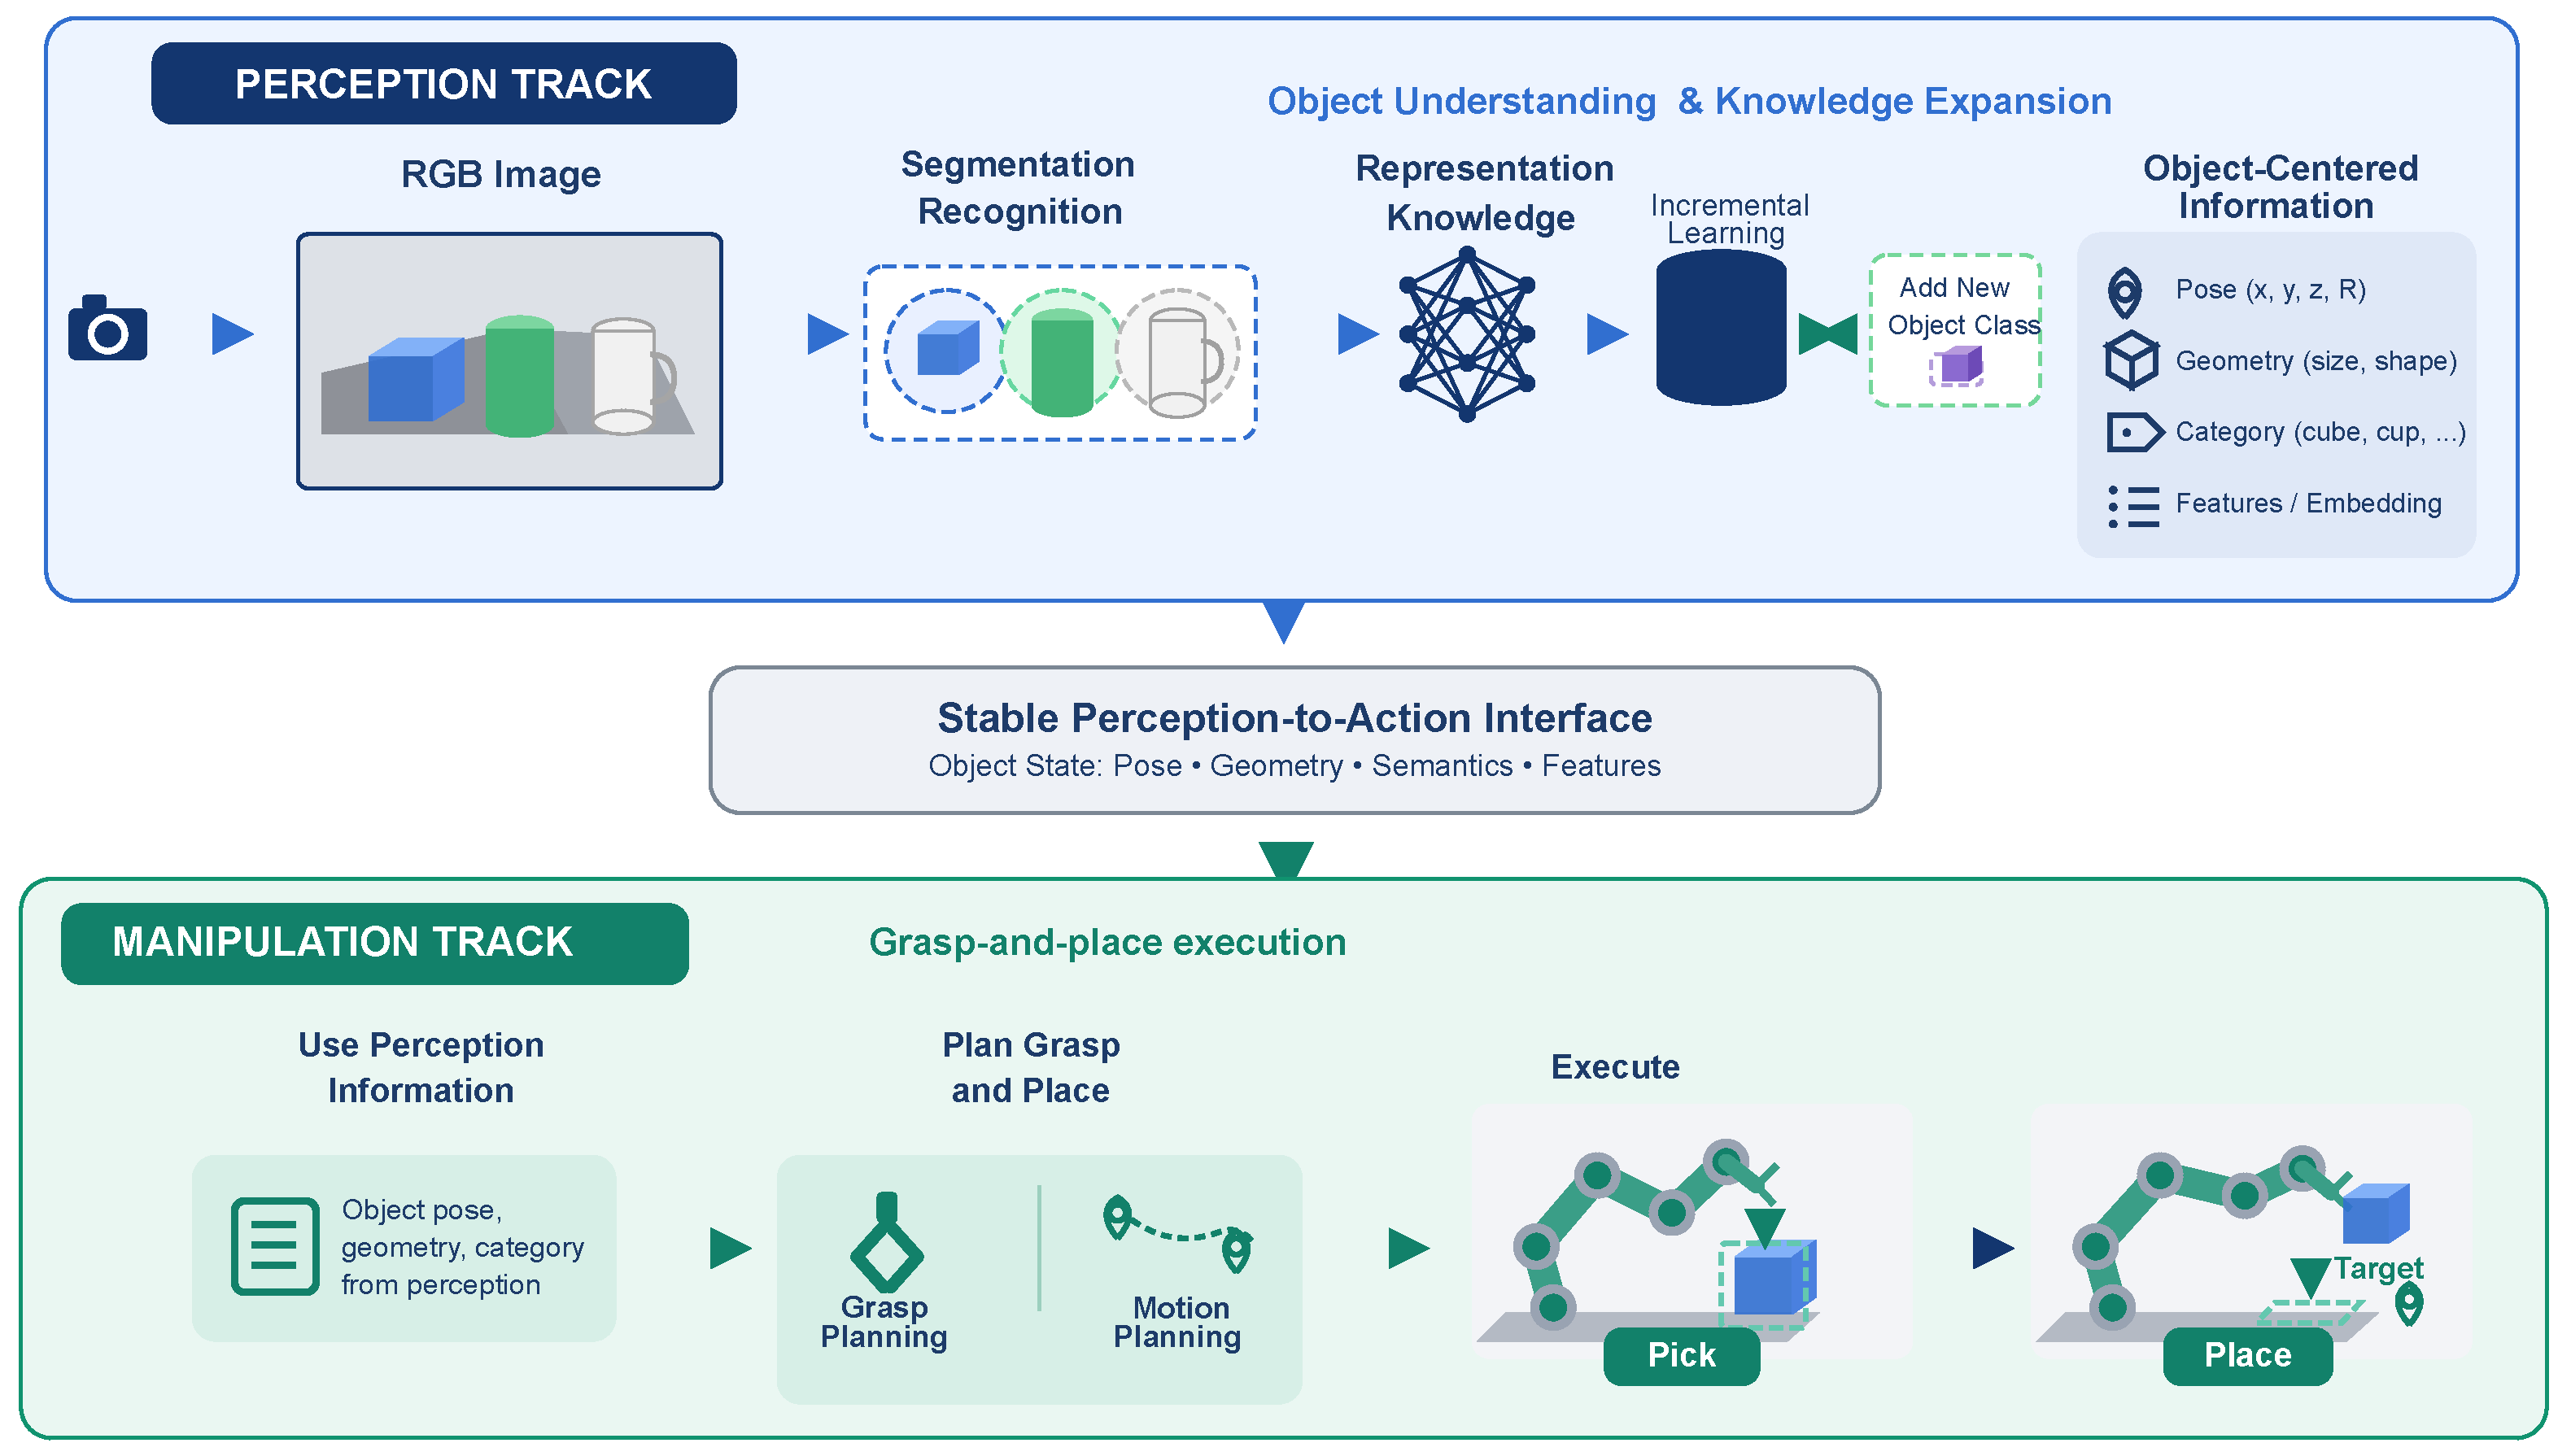
\includegraphics[width=0.5\linewidth]{assets/overall-system-diagram.pdf}
    \end{figure}

    \vspace{-0.3cm}
    \centering
    \small The proposed system connects perception and manipulation through a shared perception-to-action interface.
\end{frame}

\begin{frame}{Methodology: Key Idea}
    \small
    \begin{itemize}
        \item The long-term target is a modular visuomotor pipeline.
        \item The \textbf{perception module} estimates object-centered information and expands object knowledge over time.
        \item The \textbf{manipulation module} uses that information to generate grasp-and-place behavior.
        \item In this work, these two parts are studied separately through a perception study and a manipulation study.
        \item The long-term goal is to connect them through a stable perception-to-action interface \cite{Zheng2025EmbodiedManipSurvey,Kasaei2021LifelongServiceRobots}.
    \end{itemize}
\end{frame}

% ------------------------------------------------
\section{Manipulation}

\begin{frame}{Manipulation Objective}
\begin{block}{Goal}
Develop a tabletop pick-and-place capability for the Fourier GR-1 humanoid in simulation.
\end{block}

\begin{itemize}
    \item Initial assumption: cube position is available from simulation state.
    \item Task: grasp a cube from the table and place it at a predefined target location.
    \item Main question: how far can a scripted controller go, and where does learned control become necessary?
\end{itemize}
\end{frame}

\begin{frame}{Simulation Setup}
\begin{figure}
    \centering
    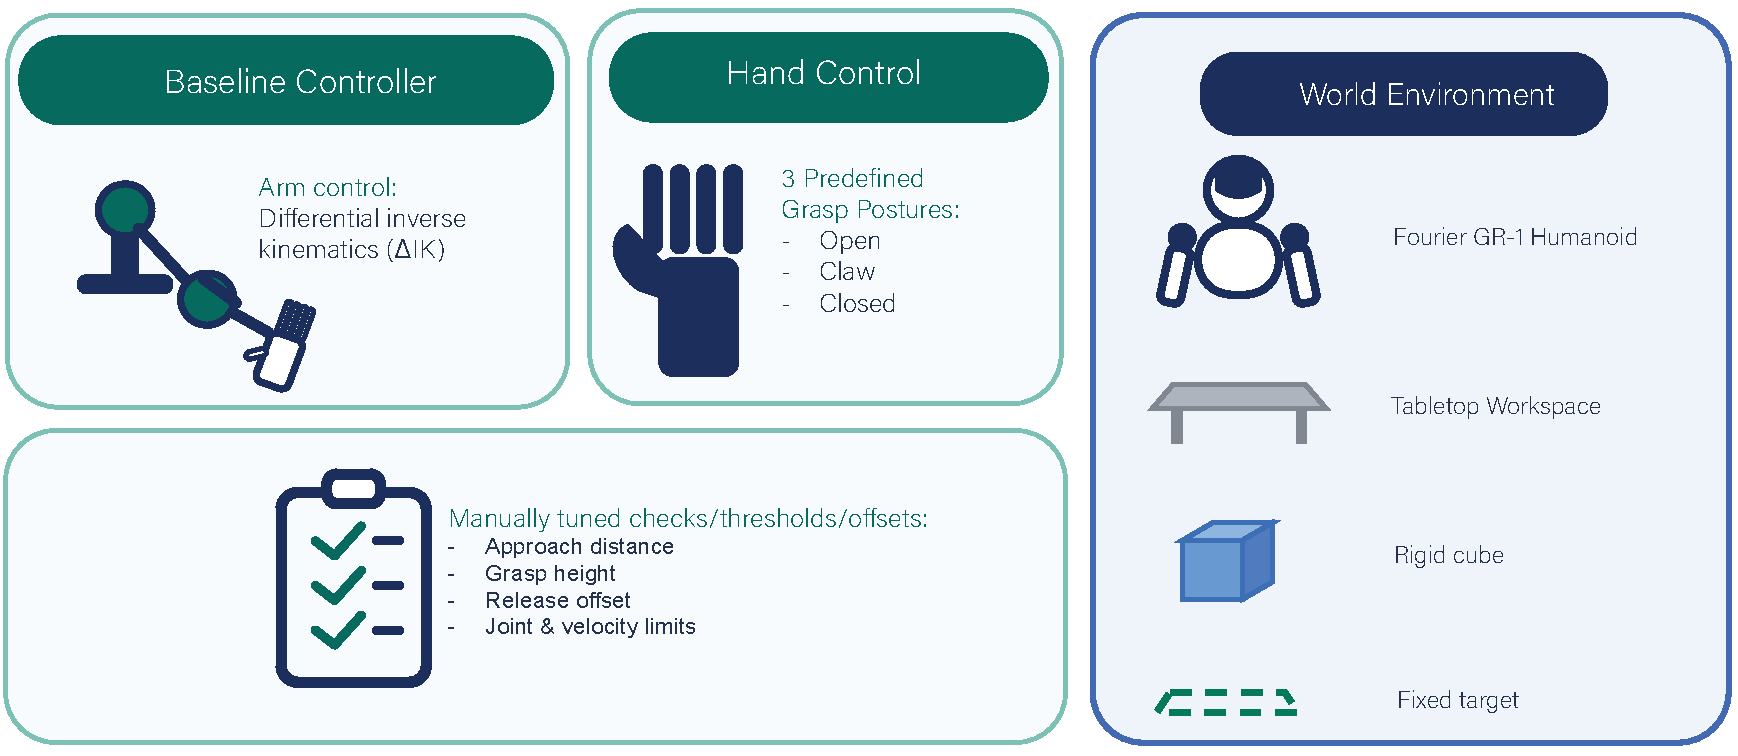
\includegraphics[width=0.9\linewidth]{assets/manipulation-diagram.pdf}
    \caption{Manipulation task environment}
    \label{fig:manipulation}
\end{figure}
\end{frame}

\begin{frame}{Scripted Baseline}
\begin{itemize}
    \item The first controller is a \textbf{hand-designed state machine}.
    \item This provides a structured and debuggable baseline for tabletop pick-and-place.
\end{itemize}
\begin{figure}
    \centering
    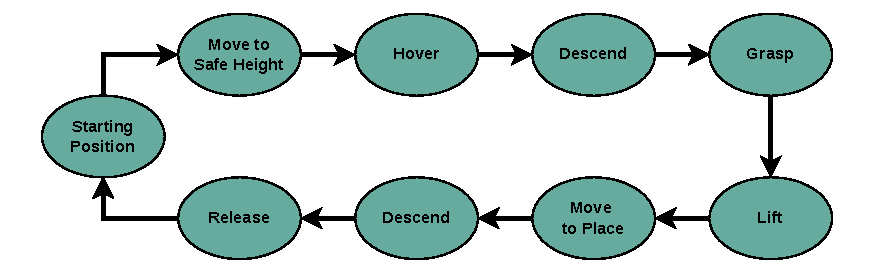
\includegraphics[width=0.9\linewidth]{assets/stagediagram.pdf}
    \caption{Stage flow diagram}
    \label{fig:stage-diagram}
\end{figure}
\end{frame}

\begin{frame}{Baseline Control Structure}
\begin{itemize}
    \item \textbf{Arm control:} differential inverse kinematics maps desired end-effector pose to arm joint targets.
    \item \textbf{Hand control:} predefined hand postures (\textit{open}, \textit{claw}, \textit{closed}).
    \item \textbf{State transitions:} based on manually designed conditions:
    \begin{itemize}
        \item XY alignment,
        \item Z alignment,
        \item hand-to-cube proximity,
        \item lift height,
        \item hold counters.
    \end{itemize}
\end{itemize}
\end{frame}

\begin{frame}{Assumptions and Constraints}
\begin{itemize}
    \item Cube position is directly available from simulator state.
    \item Placement target is predefined.
    \item End-effector orientation is fixed.
    \item Motion depends on manually tuned:
    \begin{itemize}
        \item height offsets,
        \item palm alignment biases,
        \item stage thresholds,
        \item grasp posture schedules.
    \end{itemize}
    \item Cube pose is randomized slightly across episodes, but the control strategy remains scripted.
\end{itemize}
\end{frame}

\begin{frame}{What the Baseline Provides}
\begin{block}{Value of the baseline}
It shows that the robot can perform tabletop pick-and-place under controlled assumptions.
\end{block}

\begin{itemize}
    \item Establishes the scene, robot, and control pipeline.
    \item Makes failure modes easier to inspect.
    \item Provides a reference system before learning-based control.
\end{itemize}

\vspace{0.2cm}
\begin{alertblock}{Main limitation}
The system still depends on heuristic offsets, thresholds, and predefined stage logic.
\end{alertblock}
\end{frame}

\begin{frame}{RL Reformulation}
\begin{itemize}
    \item To reduce dependence on hand-crafted stage logic, the task was reformulated as a \textbf{reinforcement learning problem}.
    \item A parallel Isaac Lab environment was created for multi-environment training.
    \item Training uses \textbf{PPO}.
    \item Goal: allow the robot to discover grasping and transport behavior through interaction rather than explicit stage scripting \cite{Kober2013RLRobotics}.
\end{itemize}
\end{frame}

\begin{frame}{RL Environment}
\begin{itemize}
    \item \textbf{Observation includes:}
    \begin{itemize}
        \item end-effector position,
        \item cube position,
        \item placement target position,
        \item relative vectors,
        \item arm joint positions,
        \item hand joint positions.
    \end{itemize}
    \item \textbf{Action includes:}
    \begin{itemize}
        \item incremental arm joint commands,
        \item one scalar grip-control signal.
    \end{itemize}
    \item Cube position is randomized at reset to avoid overfitting to a single trajectory, following the general motivation of reducing sim-specific overfitting \cite{Tobin2017DomainRandomization}.
\end{itemize}
\end{frame}

\begin{frame}{Reward Design}
\begin{itemize}
    \item Reward encourages:
    \begin{enumerate}
        \item reaching the cube,
        \item lifting the cube,
        \item transporting it toward the goal,
        \item successful placement.
    \end{enumerate}
    \item A penalty on action magnitude discourages unnecessarily aggressive control.
    \item Episodes terminate on:
    \begin{itemize}
        \item success,
        \item cube drop,
        \item out-of-bounds behavior,
        \item timeout.
    \end{itemize}
\end{itemize}
\end{frame}

\begin{frame}{Interpretation}
\begin{itemize}
    \item The manipulation work follows a clear progression:
    \begin{enumerate}
        \item establish a scripted baseline,
        \item identify brittle hand-crafted assumptions,
        \item reformulate the task as learned control.
    \end{enumerate}
    \item This study does not yet solve fully dynamic grasping.
    \item It does establish the control-side foundation required for a future integrated visuomotor pipeline \cite{Zheng2025EmbodiedManipSurvey}.
\end{itemize}
\end{frame}

% ------------------------------------------------
\section{Perception}

\begin{frame}{Perception Objective}
\begin{block}{Goal}
Develop an incremental semantic segmentation module that can learn new object classes over time while minimizing catastrophic forgetting.
\end{block}

\begin{itemize}
    \item Motivation: in open-world robotics, new objects appear after deployment \cite{Kasaei2021LifelongServiceRobots}.
    \item Full retraining is slow and impractical for continual operation.
    \item The perception module should expand object knowledge while preserving old classes \cite{Zhou2024CILSurvey}.
    \item In the long term, this module will provide object-centered information for downstream grasping and placement.
\end{itemize}
\end{frame}

\begin{frame}{Perception Flow Diagram}
\begin{figure}
    \centering
    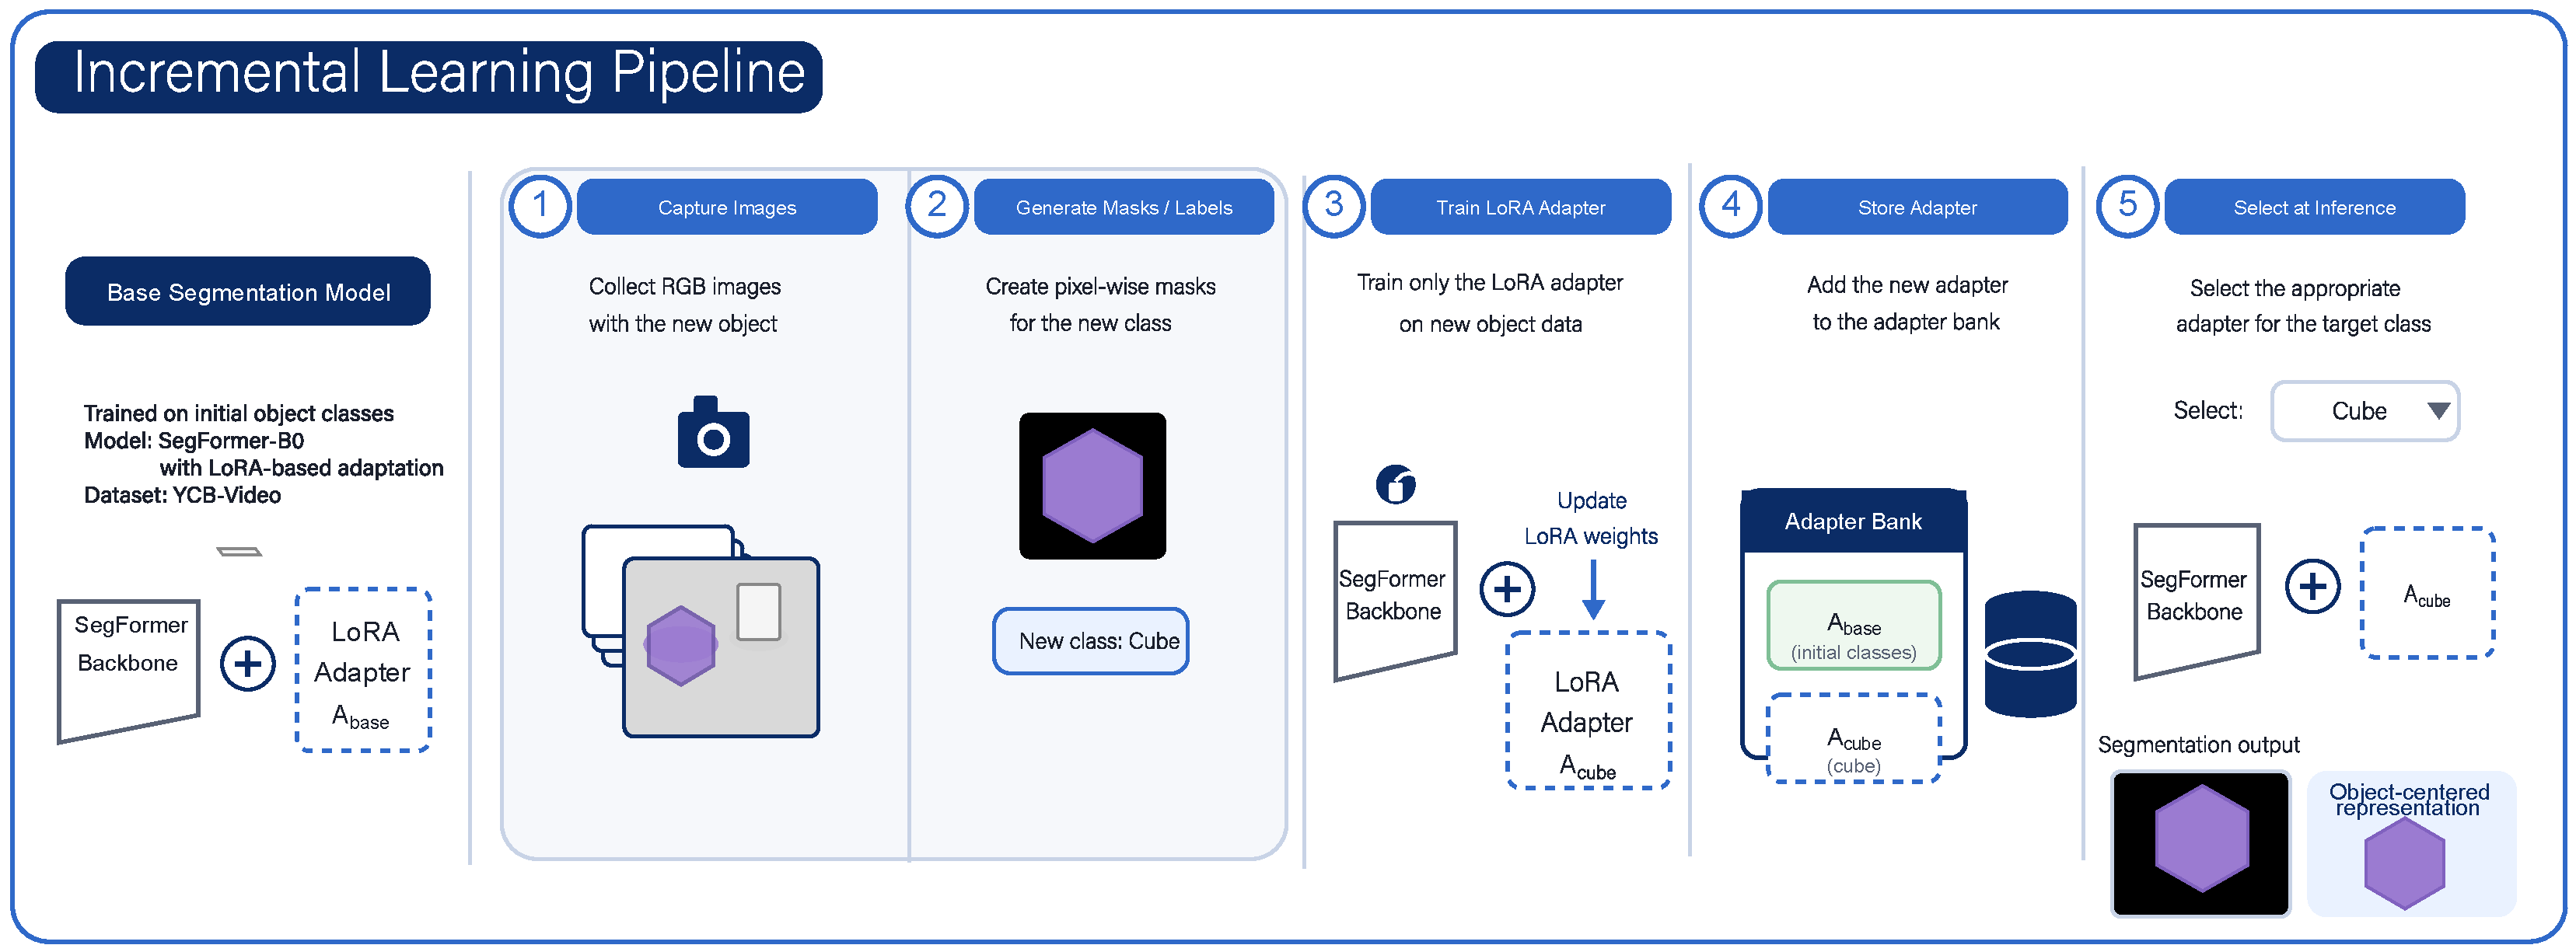
\includegraphics[width=0.6\linewidth]{assets/perception-diagram.pdf}
    \caption{Perception incremental learning pipeline}
    \label{fig:perception}
\end{figure}
\end{frame}

\begin{frame}{Proposed Pipeline}
\begin{itemize}
    \item Start with a base segmentation model trained on initial object classes.
    \item When a robot encounters a new object:
    \begin{enumerate}
        \item capture images,
        \item generate labels and masks automatically,
        \item train a new LoRA adapter,
        \item store the adapter in a library,
        \item select the correct adapter at inference.
    \end{enumerate}
    \item Long-term goal: continual perception without destroying prior knowledge \cite{Hu2021LoRA,Zhou2024CILSurvey}.
\end{itemize}

\vspace{0.2cm}
\begin{alertblock}{Current scope}
In this work, the full online robot pipeline was not implemented, so the study focuses on offline incremental segmentation experiments.
\end{alertblock}
\end{frame}

\begin{frame}{Dataset and Setup}
\small
\begin{itemize}
    \item \textbf{Dataset:} YCB-Video
    \begin{itemize}
        \item 21 household object classes,
        \item RGB-D video with pixel-level annotations,
        \item class split: base classes 1--10, new classes 11--21.
    \end{itemize}
    \item \textbf{Proof-of-concept subset:}
    \begin{itemize}
        \item 5 sequences,
        \item 6,638 usable frames,
        \item 5,974 train / 664 test.
    \end{itemize}
    \item \textbf{Model:} SegFormer-B0 with modified segmentation head.
    \item \textbf{Adaptation:} LoRA inserted into selected transformer layers \cite{Hu2021LoRA}.
    \item \textbf{Metric:} mean Intersection-over-Union (mIoU).
\end{itemize}
\end{frame}

\begin{frame}{Incremental Learning Results}
\footnotesize
\centering
\renewcommand{\arraystretch}{1.15}
\setlength{\tabcolsep}{4pt}

\begin{table}[h]
\centering
\begin{tabularx}{0.96\textwidth}{p{3.5cm} c c c}
\toprule
\textbf{Method} & \textbf{Base IoU Before} & \textbf{Base IoU After} & \textbf{New Class IoU} \\
\midrule
Naive Fine-Tuning & 0.96 & 0.18 & 0.95 \\
LoRA Fine-Tuning & 0.96 & 0.19 & 0.93 \\
Adapter Fusion & 0.96 & 0.97 & 0.42 \\
LoRA + Distillation & 0.96 & 0.8833 & 0.9144 \\
\bottomrule
\end{tabularx}
\end{table}

\vspace{0.15cm}
\begin{itemize}
    \item Naive and plain LoRA fine-tuning learned new classes but forgot old ones, consistent with catastrophic forgetting in sequential learning \cite{McCloskey1989Catastrophic,French1999Catastrophic}.
    \item Adapter fusion preserved old knowledge but underfit the new classes.
    \item \textbf{LoRA + knowledge distillation gave the best balance} between retention and new-class learning, matching the intuition behind LwF-style retention mechanisms \cite{LiHoiem2016LwF,Hu2021LoRA}.
\end{itemize}
\end{frame}

% ------------------------------------------------
\section{Status and Next Steps}

\begin{frame}{Manipulation Progression}
\scriptsize
\centering
\renewcommand{\arraystretch}{1.3}

\begin{table}[h]
\centering
\resizebox{\textwidth}{!}{%
\begin{tabular}{l l L{2.3cm} L{2.3cm} L{2.3cm} L{2.3cm} L{2.3cm}}
\toprule
\textbf{Domain} & \textbf{Capability} & \textbf{Level 0} & \textbf{Level 1} & \textbf{Level 2} & \textbf{Level 3} & \textbf{Level 4} \\
& & \textit{(Hard-coded)} & \textit{(Reactive)} & \textit{(Adaptive)} & \textit{(Autonomous)} & \textit{(Dynamic)} \\
\midrule
\textbf{Manipulation} & \textbf{Grasp Planning}
& None
& \cellcolor{blue!10}Model-based (Stage 2)
& \cellcolor{blue!25}Model-free isolated (Stage 3)
& Model-free cluttered
& Articulated / deformable \\

& \textbf{Execution}
& \cellcolor{gray!20}Hard-coded (Stage 1)
& Reactive single-modal
& \cellcolor{blue!25}Reactive multimodal (Stage 3)
& \cellcolor{blue!40}Autonomous under uncertainty (Target)
& Autonomous dynamic \\
\bottomrule
\end{tabular}%
}
\end{table}

\vspace{0.1cm}
\textbf{Reading:} The current system moves from a hard-coded baseline toward a model-free RL policy as the next major capability step.
\end{frame}

\begin{frame}{Perception Progression}
\scriptsize
\centering
\renewcommand{\arraystretch}{1.3}

\begin{table}[h]
\centering
\resizebox{\textwidth}{!}{%
\begin{tabular}{l l L{2.35cm} L{2.35cm} L{2.35cm} L{2.35cm} L{2.35cm}}
\toprule
\textbf{Domain} & \textbf{Capability} & \textbf{Level 0} & \textbf{Level 1} & \textbf{Level 2} & \textbf{Level 3} & \textbf{Level 4} \\
& & \textit{(Static)} & \textit{(Offline Incremental)} & \textit{(Retention-Aware)} & \textit{(Online Adaptive)} & \textit{(Embodied Continual)} \\
\midrule
\textbf{Perception} & \textbf{Object Knowledge}
& Fixed class set
& \cellcolor{blue!10}Offline class-incremental updates
& \cellcolor{blue!25}LoRA + distillation retention
& Online novel-class expansion
& Continual open-world object learning \\

& \textbf{System Integration}
& Standalone segmentation
& Dataset-level evaluation
& \cellcolor{blue!25}Incremental method comparison
& On-robot perception updates
& \cellcolor{blue!40}Perception-action integration (Target) \\
\bottomrule
\end{tabular}%
}
\end{table}

\vspace{0.1cm}
\textbf{Reading:} The current perception system has moved beyond static segmentation into offline incremental learning, with LoRA + distillation as the strongest retention-aware baseline.
\end{frame}

\begin{frame}{Next Steps}
\begin{itemize}
    \item On the perception side, move from offline incremental segmentation toward online novel-class adaptation and robot-level integration \cite{Kasaei2021LifelongServiceRobots,Meng2025RoboticLifelongRL}.
    \item On the manipulation side, improve the RL policy until grasping is more robust to pose variation.
    \item Reduce reliance on fixed offsets and predefined stage assumptions in manipulation.
    \item Integrate the perception and manipulation modules into a single visuomotor pipeline.
    \item After stable simulation performance, transfer the integrated system to the physical Fourier GR-1 robot.
\end{itemize}
\end{frame}

% ------------------------------------------------
\section{Conclusion}

\begin{frame}{Conclusion}
\begin{itemize}
    \item This work targets a foundational robotics problem: tabletop perception-to-manipulation with a humanoid robot \cite{Zheng2025EmbodiedManipSurvey}.
    \item The current contribution on the manipulation side is a progression from scripted control to RL-based adaptive control.
    \item The perception-side contribution is an incremental segmentation study showing that LoRA + distillation gives the strongest retention/plasticity trade-off in the current setup \cite{LiHoiem2016LwF,Hu2021LoRA}.
    \item Together, these studies establish the basis for a larger integrated visuomotor system.
\end{itemize}
\end{frame}

\begin{frame}[allowframebreaks]{References}
\scriptsize
\bibliographystyle{alpha}
\bibliography{references}
\end{frame}

\begin{frame}{Thank You}
  \centering
  \Huge Questions?
\end{frame}

\end{document}